% Sources :
%	http://forum.mathematex.net/post89969.html
%	http://forum.mathematex.net/latex-f6/tikz-et-alignement-de-nodes-t12454.html#p120743

\documentclass[10pt,a4paper]{article}
	\usepackage[utf8x]{inputenc}
	\usepackage{ucs}
	\usepackage{tikz}
	\usepackage{amsmath}


\begin{document}

Matrice de type ''carré'' :

\[
	\begin{pmatrix}
		\begin{tikzpicture}
			\node (a) at (0,0) {a \vphantom{b}};
			\node (b) at (1,0) {b};
			\node (c) at (0,-1) {c \vphantom{d}};
			\node (d) at (1,-1) {d};

			\draw (a.east) -- (b.west);
			\draw (b.south) -- (d.north);
			\draw (c.east) -- (d.west);
			\draw (a.south) -- (c.north);
		\end{tikzpicture}
	\end{pmatrix}
\]


Matrice de type ''carré-diagonale'' :

\[
	\begin{pmatrix}
		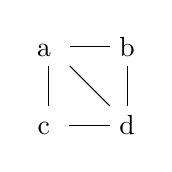
\begin{tikzpicture}
			\node (a) at (0,0) {a \vphantom{b}};
			\node (b) at (1,0) {b};
			\node (c) at (0,-1) {c \vphantom{d}};
			\node (d) at (1,-1) {d};

			\draw (a.east) -- (b.west);		
			\draw (b.south) -- (d.north); 
			\draw (c.east) -- (d.west); 
			\draw (a.south) -- (c.north); 
			\draw (a.south east) -- (d.north west);		 
		\end{tikzpicture}
	\end{pmatrix}
\]


Matrice de type ''2-triangles-diagonale'' :

\[
	\begin{pmatrix}
		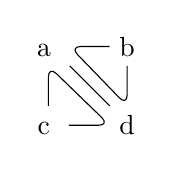
\begin{tikzpicture}
			\node (a) at (0,0) {a \vphantom{b}};
			\node (b) at (1,0) {b};
			\node (c) at (0,-1) {c \vphantom{d}};
			\node (d) at (1,-1) {d};

			\draw (a.south east) -- (d.north west); % Diagonal
			\draw [rounded corners] (b.south)--(d.north)--(a.east)--(b.west); % Lower triangle 
			\draw [rounded corners] (c.north)--(a.south)--(d.west)--(c.east); % Upper triangle 
		\end{tikzpicture}
	\end{pmatrix}
\]


Amélioration de la gestion de l'alignement :

\[
	\begin{pmatrix}
		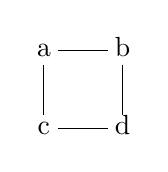
\begin{tikzpicture}
			\node[minimum size=1em] (a) at (0,0)  {};
			\node[minimum size=1em] (b) at (1,0)  {};
			\node[minimum size=1em] (c) at (0,-1) {};
			\node[minimum size=1em] (d) at (1,-1) {};

			\begin{scope}[every node/.style={anchor=mid}] 
				\node  at (0,0)  {a};
				\node  at (1,0)  {b};
				\node  at (0,-1) {c};
				\node  at (1,-1) {d};
			\end{scope}

			\draw (a) -- (b);
			\draw (b) -- (d);
			\draw (c) -- (d);
			\draw (a) -- (c);
		\end{tikzpicture}
	\end{pmatrix}
\]

\end{document}